\pagenumbering{arabic}
\section{Problem formalisation}
This project is about retrieving data in range without allowing the server to read it, and also to relate the queries and the nodes in memory. 
Basically, our goal is to build a database that allows the client to maintain the confidentiality of the data stored, despite all the data is stored in a different location from the client's hard disk. This means that all the data written on the hard disk can be easily read by another person who can do anything with it. 
Given that, we need to encrypt that data from eavesdroppers or other people. This is because they could sell it or login into accounts and use them for stealing money or identities. In order to achieve this, we need to encrypt the data stored in the hard drive, so that only the one who has the key can easily read the information stored, while all the others are going to read only encrypted data.
Obviously, according to that, all the data management must be done by the client, otherwise any malicious person can easily retrieve it and use it for any malicious intention.
The first chapter concerns about introducing the structures used for the realization of the project and some technical terms necessary for the second part.
\\
The second chapter examines various encrypted databases, and explain the methods that they use for realize such purpose.
\\
The third chapter concerns about the implementation of the project and its details.
\\In the fourth chapter there is the testing of the project over some databases.
\\Concluding the last chapter explain the results obtained and the future work based on this project, with some possible uses of it.

%(the server retrieve what? And the server use it for bad purposes? This last sentence needs to be reviewed. Apart from this, now the English is quite good. You should explain more than "why we need to encrypt the data" how you retrieve data in range, since as I understood it's the main part of the thesis!

\section{Background knowledge}
\subsection{B+tree}
A B+tree is a data structure used for ordering the keys in a database. Each node has a large number of children. They are used in many contexts, from filesystems, like NTFS, to databases. It is indexed on a single key and, differently from a standard binary tree, all the data is stored under the leaves, as it is shown in figure 1. This means that, if we want to retrieve a record from this database, we have a complexity of $o(h)$ where $h$ is the height of the tree. 
The root and the internal node have more than $\frac{n}{2}$ children, where $n$ is the maximum number of children that a node can have. All the data under the leaves is linked by a pointer that points to the record. %with that key
%In each internal node, all the keys %that between the searched key is located between the nearest pointers (one lower and one higher). 
Searching the specified key on this data structure can be easily made by following the path denoted by the keys in the internal nodes. It has a complexity of $O(\log{} _a n)$, where a is the branching factor of the tree and n is the height of the tree (defined as the number of levels in the tree).
In our implementation we don't have any link between the leaves, that means we have to start from the parent for retrieve any sibling of the node, and also we have to start from the root to do range queries. We used this implementation because in order to to preserve the tree we need to keep in memory all the nodes between the root and the current, so that each node we retrieve, including the ones recovered from fake searches, must be attainable from the root.
  %not only that for retrieve every leaf we must begin from the parent but also a different approach for do a range query.
\\

\begin{figure}[htbp]
\centering
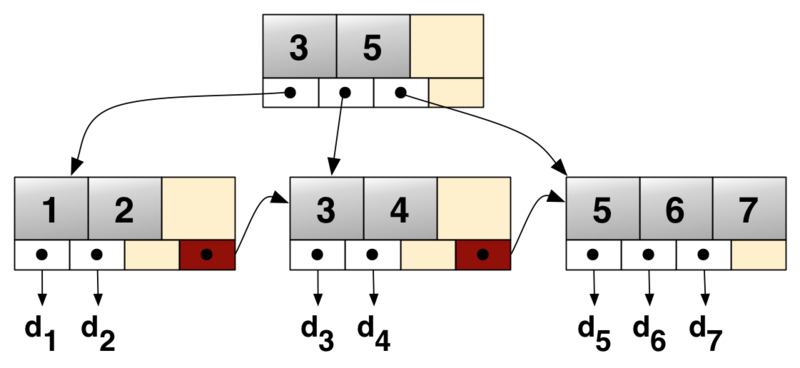
\includegraphics[scale=0.8]{bplustree.png}
\\Figure 1: A graphical representation of a b+tree (source www.wikipedia.org)
\end{figure}
\newpage
\subsection{AES algorithm}
The AES algorithm (also called Rijndael from its creators Vincent Rijmen and Joan Daemon), is a symmetric encryption algorithm. Symmetric means that the same key is used both for encrypting and decrypting. It became effective in 2002, after the approval of NIST. This algorithm is a block chiper, i.e. it processes blocks of fixed length (128 bit) arranged on a matrix (called \textbf{State Array}) where the first word (each word is four bytes) is in the first column and so on. 
$State Array = 
\begin{bmatrix}
s_{0,0} & s_{0,1} & s_{0,2} & s_{0,3} \\ 
s_{1,0} & s_{1,1} & s_{1,2} & s_{1,3} \\
s_{2,0} & s_{2,1} & s_{2,2} & s_{2,3} \\
s_{3,0} & s_{3,1} & s_{3,2} & s_{3,3} \\
\end{bmatrix}
$
The algorithm is composed of k rounds (as it is shown in figure 2) where k  depends on the key length. In our case we have a 128 bit key, that means AES standard, therefore we have k equal to 10 plus the first add round key  (in case of 196 bits k is 12 and 14 in case of 256 bits key).
\newpage
\begin{figure}[htbp]
\centering
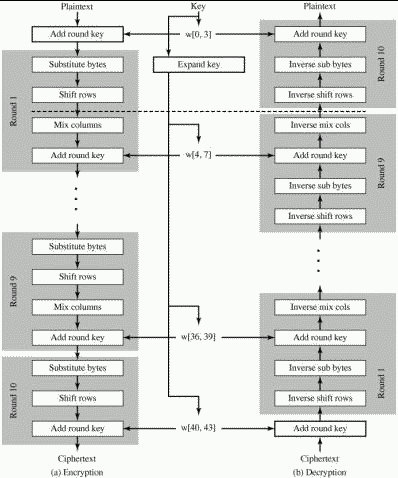
\includegraphics[scale=1]{AES_structure.png}
\\Figure 2: AES structure (source http://www.codeproject.com)
\end{figure}

\subsection{Key expansion algorithm}

Before applying the algorithm the key must be expanded, because at each step the add round key needs a portion of it. It is designed to ensure that a minimum change in the key (just only one bit is enough) should affect the next round keys for several times. A 128 bit key is expanded in the following manner: 
First is divided in 4 words as below:
\newpage

\begin{center}
$\begin{bmatrix}
k_0 & k_1 & k_2 & k_3\\
k_4 & k_5 & k_6 & k_7\\
k_8 & k_9 & k_10 & k_11\\
k_12 & k_13 & k_14 & k_15\\
\end{bmatrix}$\\
$\Downarrow$\\
$
\begin{bmatrix}
w_0 & w_1 & w_2 & w_3
\end{bmatrix}$\\
\end{center}
After this step the algorithm proceed four word at a time, as it is shown below in figure 4.\\
\begin{figure}[htbp]
	\centering
	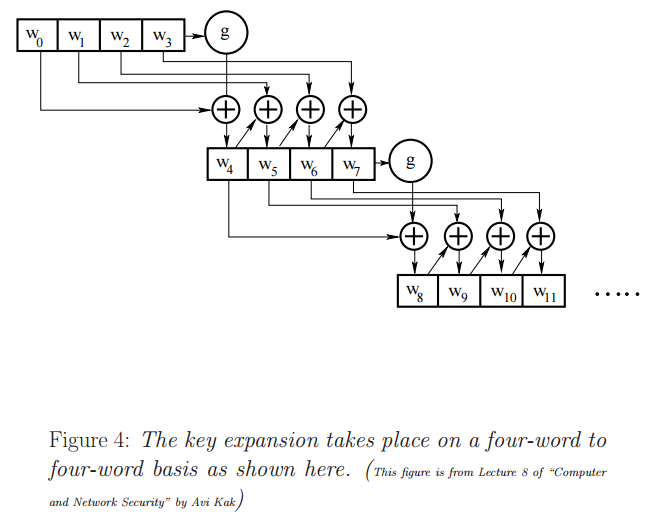
\includegraphics[scale=0.7]{key_expansion.png}
\end{figure}
\\Where $\oplus$ is the addition modulus 2 between the bits of the words and $g$ is a mathematical function as below.
$g()$ is composed by 3 steps: 
\begin{enumerate}
	\item One-byte left circular rotation on the 4 byte word.
	\item Byte substitution for each byte of the word returned using the lookup table taken from the Substitute Bytes step.
	\item XOR the bytes obtained from the previous step with a round constant. This step is important to destroy any symmetry that can exists in the previous steps.\\
	The round constant is derived at each round with the following formula (i starting from 1 is the number of the round):\\
	$Rcon[i] = (RC[i], 0x00, 0x00, 0x00)$\\
	Where:\\
	$RC[1] = 0x01$\\
	$RC[j] = 0x02 \times RC[j-1]$
\end{enumerate}


\subsubsection{Encryption}
Each round, except for the first (that is only an add round key) and the last, is composed by 4 steps:
\begin{enumerate}
\item substitute bytes
\item shift rows
\item mix columns
\item add round key
\end{enumerate}

The last round doesn't have the mix columns step in order to make the algorithm reversible. 
\paragraph{Substitute Bytes: }
The bytes substitution in the encryption works by replacing each byte with the corresponding value in the S-BOX, that is a $16\times16$ matrix (as it is shown below in figure 3). The lookup table is shown in hexadecimal value.
\newpage
\begin{figure}[htbp]
\centering
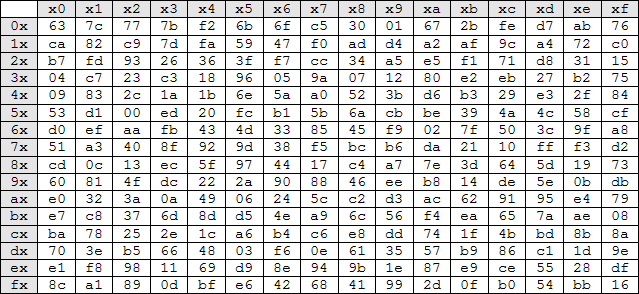
\includegraphics[scale=0.7]{sbox.png}
\\Figure 3: S-BOX (source https://edipermadi.wordpress.com)
\end{figure}
In this step the lookup table cannot be described as a mathematical function so the algorithm has to access the table every time.\\


\paragraph{Shift Rows: }
During the shift rows step each row of the state array is shifted as following:\\
\begin{center}
$
\begin{bmatrix}
s_{0,0} & s_{0,1} & s_{0,2} & s_{0,3} \\ 
s_{1,0} & s_{1,1} & s_{1,2} & s_{1,3} \\
s_{2,0} & s_{2,1} & s_{2,2} & s_{2,3} \\
s_{3,0} & s_{3,1} & s_{3,2} & s_{3,3} \\
\end{bmatrix}
\implies
\begin{bmatrix}
s_{0,0} & s_{0,1} & s_{0,2} & s_{0,3} \\ 
s_{1,1} & s_{1,2} & s_{1,3} & s_{1,0}\\
s_{2,2} & s_{2,3} & s_{2,0} & s_{2,1} \\
s_{3,3} & s_{3,0} & s_{3,1} & s_{3,2} \\
\end{bmatrix}
$
\end{center}
\paragraph{Mix Columns}
The mix columns step is composed by four operations, one for each row of the state array, as it is shown below:

\begin{itemize}
	\item For the first row the operation can be stated as: 
	$s'_{0,j} = (0x02 \times s_{0,j}) \otimes (0x03 \times s_{1,j}) \otimes s_{2,j} \otimes s_{3,j})$
	\item For the second row the operation can be stated as: 
	$s'_{1,j} = s_{0,j} \otimes (0x02 \times s_{1,j}) \otimes (0x03 \times s_{2,j}) \otimes s_{3,j})$
	\item For the third row the operation can be stated as: 
	$s'_{2,j} = s_{0,j} \otimes s_{1,j} \otimes (0x02 \times s_{2,j}) \otimes (0x03 \times s_{3,j}))$
	\item For the fourth row the operation can be stated as: 
	$s'_{3,j} = (0x03 \times s_{0,j}) \otimes s_{1,j} \otimes s_{2,j} \otimes (0x02 \times s_{3,j}))$
\end{itemize}

Or more compactly:
$
\begin{bmatrix}
02 & 03 & 01 & 01 \\ 
01 & 02 & 03 & 01 \\
01 & 01 & 02 & 03 \\
03 & 01 & 01 & 02 \\
\end{bmatrix}
\times
\begin{bmatrix}
s_{0,0} & s_{0,1} & s_{0,2} & s_{0,3} \\ 
s_{1,0} & s_{1,1} & s_{1,2} & s_{1,3} \\
s_{2,0} & s_{2,1} & s_{2,2} & s_{2,3} \\
s_{3,0} & s_{3,1} & s_{3,2} & s_{3,3} \\
\end{bmatrix}
=
\begin{bmatrix}
s'_{0,0} & s'_{0,1} & s'_{0,2} & s'_{0,3} \\ 
s'_{1,0} & s'_{1,1} & s'_{1,2} & s'_{1,3} \\
s'_{2,0} & s'_{2,1} & s'_{2,2} & s'_{2,3} \\
s'_{3,0} & s'_{3,1} & s'_{3,2} & s'_{3,3} \\
\end{bmatrix}
$

\paragraph{Add round key}

The add round key step is done by XORing each byte of the state with the relative byte of the key expanded. In the first round the input block is XORed with the first 4 words of the expanded key, and then at each of the following rounds the block is XORed with the next 4 words at a time.

\subsubsection{Decryption}
Each round, as it works in the encryption, is composed by 4 steps (first add round key and last round excluded):
\begin{enumerate}
\item substitute bytes
\item shift rows
\item mix columns
\item add round key
\end{enumerate}
\paragraph{Inverse Substitute Bytes: }
Like in the encryption, the bytes substitution is made by replacing every byte with the corresponding value. Differently from the encryption the value is searched in the inverse S-BOX (as it is shown below in figure 4).

\begin{figure}[htbp]
\centering
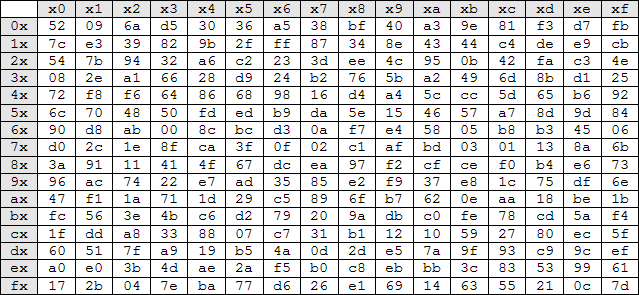
\includegraphics[scale=0.7]{isbox.png}
\\Figure 4: Inverse S-BOX (source https://edipermadi.wordpress.com)
\end{figure}

\paragraph{Shift rows}
During the shift rows step each row of the state array is shifted as following:\\
\begin{center}
	$
	\begin{bmatrix}
	s_{0,0} & s_{0,1} & s_{0,2} & s_{0,3} \\ 
	s_{1,0} & s_{1,1} & s_{1,2} & s_{1,3} \\
	s_{2,0} & s_{2,1} & s_{2,2} & s_{2,3} \\
	s_{3,0} & s_{3,1} & s_{3,2} & s_{3,3} \\
	\end{bmatrix}
	\implies
	\begin{bmatrix}
	s_{0,0} & s_{0,1} & s_{0,2} & s_{0,3} \\ 
	s_{1,3} & s_{1,0} & s_{1,1} & s_{1,2}\\
	s_{2,2} & s_{2,3} & s_{2,0} & s_{2,1} \\
	s_{3,1} & s_{3,2} & s_{3,3} & s_{3,0} \\
	\end{bmatrix}
	$
\end{center}
\paragraph{Mix columns}


The mix columns step is composed by four operations, one for each row of the state array, as it is shown below:

$
\begin{bmatrix}
0E & 0B & 0D & 09 \\ 
09 & 0E & 0B & 0D \\
0D & 09 & 0E & 0B \\
0B & 0D & 09 & 0E \\
\end{bmatrix}
\times
\begin{bmatrix}
s_{0,0} & s_{0,1} & s_{0,2} & s_{0,3} \\ 
s_{1,0} & s_{1,1} & s_{1,2} & s_{1,3} \\
s_{2,0} & s_{2,1} & s_{2,2} & s_{2,3} \\
s_{3,0} & s_{3,1} & s_{3,2} & s_{3,3} \\
\end{bmatrix}
=
\begin{bmatrix}
s'_{0,0} & s'_{0,1} & s'_{0,2} & s'_{0,3} \\ 
s'_{1,0} & s'_{1,1} & s'_{1,2} & s'_{1,3} \\
s'_{2,0} & s'_{2,1} & s'_{2,2} & s'_{2,3} \\
s'_{3,0} & s'_{3,1} & s'_{3,2} & s'_{3,3} \\
\end{bmatrix}
$

\paragraph{Add round key}
The add round key step in the decryption is the same as the encryption.


